\chapter{Analysis}\label{chap:analysis}
\section{What is music? Audiation:} \todo{Cut from this into the introduction.}
\todo{The whole section needs alot of cites}
\todo{jeg synes mange af de info der er her (hele begrebet audiation) går i glemmebogen, det bliver ikke nævnt eller brugt overhoved nogle andre steder. - Hvorfor ? og skal de så væk, eller skal vi få det inkluderet ? }
\begin{quote}
	\textit{Sound itself is not music. Sound becomes music through audiation, when, as with language, you translate sounds in your mind and give them meaning.} \cite{audiation}\\
\end{quote}

Everyone has a meaning about the sound they hear, and the meaning differs from individual to individual.\cite{audiation} Audiation is the concept of assimilating and comprehending music heard by the individual, either in the present or in the past. We can also audiate through reading notations, composing contemporary music or improvising on an instrument.
The concept of audiation is similar to the concept of language\cite{audiation}: \\

\begin{quote}
	\textit{"Consider language, speech and thought. Language is the result of the need to communicate. Speech is the way we communicate. Thought is what we communicate. Music, performance and audiation have parallel meanings. Music is the subject of communication. Performance is the vehicle for communication. Audiation is what is communicated."} \cite{audiation}\\
\end{quote}

An individual can begin audiating shortly after hearing music, to give meaning to the sound. What the individual can take from the audiation depends on that particular individuals previous audiation.\cite{audiation} The concept is similar to regular conversation – if a group of people are talking, each individual will take their own comprehension of the conversation with them. This comprehension is based on existing knowledge and experience on the topic.\cite{audiation} 
The concept of audiation increases the chance of remembering what the individual learns long term. Everyone can remember 7 +/- 2 things\todo{Get a reference}, however, if the individual tries to remember something without comprehending it, it quickly slips away again. If students have issues with vocal or instrumental techniques, or they struggle with memory lapses, it is most likely due to them not auditing while playing or singing. If the student audiates away from their instrument, it can correct technical and memory issues, including issues related to tone. Audiating before performing sound is key to learning music. Instruments should not be seen as the tool to learn how to understand music, but rather the tool to express the music\cite{audiation}:\\

\begin{quote}
	\textit{“Just as a calculator becomes a crutch for students who cannot multiply or divide, so music instruments become crutches for students who cannot audiate. This is immediately obvious when students learn to play scales by memorizing fingerings. Although students may recognize they are performing with poor intonation or inaccurate rhythm, their lack of audiation is virtually impossible for them to correct those problem by themselves. Audiation may be expressed through a music instrument, but it cannot be taken from a music instrument.”} \cite{audiation} \\
\end{quote} 

Audiation potential itself cannot be taught but rather depends on how natural musical aptitude comes to the individual. However, while Audition potential cannot be taught, students can be taught how to maximize their music achievement\cite{audiation}:\\

\begin{quote}
	“By providing children and students with appropriate knowledge and experiences, they can be taught how to audiate, that is, how to use inherent audiation as determined by their music aptitude, to maximize acquired music achievement as determined by the quality of a particular educational environment.”\cite{audiation}\\
\end{quote}
\todo{ er Der ikke lige lovlig mange citater i det her afsnit?}

The issues become evident if the students don’t learn audiation, notation and music theory in the proper sequence, they will be unable to make sense and add meaning \todo{to the sound?}the sound and music they hear or the notations they read. It is particularly evident with wind instruments Techniques refer to the methods the teacher uses to teach as well as the tools applied to achieve certain goals in different activities.\cite{audiation} If the students are unable to tonally audiate what they see in the notations, but still manipulate the keys or valves on the instrument as the notation instructions, the student will often fall out of tune.
Everyone can learn some degree of music. Similar to how everyone has at least some amount of intelligence, everyone has some amount of music aptitude, so put in other words, everyone is musical. Everyone is capable of learning to listen to and perform music to some extent of success.\cite{audiation} Generally, two-thirds of humans are average – that includes average music aptitude.
Also it is important to get students of to a good start. The foundation that is created in the early ages is a substantial influence on the music achievement of the student. Most likely, the guidance received in the early stages of their musical careers is a bigger influence, than the guidance the students receive in the higher grades or at colleges and universities. If the students musical skill-set is not properly maintained, they will severely decrease over time.
In order to maintain the skill-set properly, the techniques used by teachers have to be considered as
they are highly important. \cite{audiation}When it comes to tonation, the rhythm patterns and harmonic patterns are the most prevalent materials and they’ve remained similar for a long time across different nationalities and cultures as they belong to the basics of audiation. On the opposite side, we have activities that include larger classrooms. These will vary a lot depending on the culture, age and experience.\cite{audiation}\\


\section{Why learn music? The impact of musical education}
Several studies have shown that different types of musical engagement in a variety of ways over a lifespan has an impact on several aspects of personal growth and development. As concluded in the article "The power of music: Its impact on the intellectual, social and personal development of children and young people":\\

\begin{quote}
	\textit{"This overview provides a strong case for the benefits of active engagement with music throughout the lifespan"}\cite{powerOfMusic}\label{quote:powerOfMusic}.\\
\end{quote}

Linguistic abilities and musical training seems to be linked, due to shared brain mechanisms being used to process music and language. Precision in the perception of speech related contrasts, in pitch patterns and other distinctive speech elements have been reported to be associated with musical ability\cite{languageSkills}.\\

A study focused on literary skills showed that a group of second grade students(n = 47) taking piano lessons over a 3-year period had significantly better vocabulary and verbal abilities than a group of control students(n = 57) that did not receive music lessons\cite{vocabularySkills}.\\

Some aspects of mathematical skills have also been shown to be improved by musical training. For example the subdivision process required to read and play from music scores in order to play and keep a rhythm\cite{powerOfMusic}.\\

Other abilities have also been reported to be affected by musical training such as creativity, social and personal development, physical development, health and wellbeing\cite{powerOfMusic}.\\

According to the article \textit{Interactive music video games and children's musical development} there are 5 basic music elements that should be learned in order to get a good understanding and appreciation of music\cite[p.~99]{interactiveMusicVideoGames}:
\begin{itemize}\label{list:basicMusic}
	\item Duration
	\item Pitch
	\item Tone color
	\item Dynamics
	\item Structure\\
\end{itemize}

In another study, which focused on integration of music in the elementary classroom, results were positive. Musical activities activate both the analytical and creative side of the brain, and learning other subjects becomes easier with the addition of a musical element, as the speed at which information is processed increases. An example of this is learning the math of money exchange through music note denotations\cite{musicIntegration}.\\

Through the initial research, it can be assumed that musical education is important for the development of young students in many facets of life. In order to establish how music is learned, some research on learning in general will have to be made.

\section{Learning}
\todo{ vi har snakket om det her før, så det skal altså rettes nu. Active og passive learning bliver præsenteret dårligt i forhold til struktur. vi hører først at active learning er vejen frem ser stattestikker på både passiv og active og først bagefter bliver passive forklaret (og dersuden virker det bare underligt at skrive " det her( som faktisk allerede er blevet forklaret) er passiv lærring og det er en rigtig dårlig måde at lære på - slut " ). omskrukturer og eventuelt sammenskriv/ forklar samtidig (da de lidt er modsætninger) active og passive learning}
\subsection{Learning Defined}\label{sec:learning}
Learning is the process described as obtaining or modifying knowledge\todo{Where? Cite.}. The ability to learn exists for most living things i.e humans, animals, plants and some machines\todo{Cool, cite.}. \\
\\
There are many types of learning,\todo{jeg er ret nysgerrig nu, fortæl gerne lige hvilke andre former der findes (til mig(Sofie) ihvertfald)}
this report will mainly focus on Active Learning and Passive Learning due to being the main types of learning, when talking about education\todo{Cool, cite.}.

\subsection*{Active Learning}\label{sec:activeLearning}
Active learning comes from a person taking control of their own learning experience. If a student just sits and listens, they will not achieve as much of their learning experience as possible\todo{Cool, cite.}. Active learning comes to play, when the student actively does more than listen. They read, write discuss and engages themselves at the given topic. This also includes doing excersices and solving topic specific problems\cite{activelearning}. The use of active learning in a classroom is vital to improve the learning experience of the students. Furthermore, when not using active learning, up till 70\% of the obtained knowledge is lost within the next 24 hours \cite{learning}.\\

The retention of learning is the concept describing the processed information traveling from the short term memory to the long term memory\todo{Cool, cite.}. Furthermore, retention of learning describes how processed information can be forgotten\todo{Cool, cite.}. As aforementioned attending a lecture without actively participating except listening, can cause a person to lose the majority of information obtained withing 24 hours\todo{Cool, cite.}. Multiple theories within the retention of learning also suggests that the information is not lost, but a person is just unable to recall the information \cite{retention}.
In \autoref{fig:activelearn} the concept of retention of learning is displayed. The figure displays how different ways of learning affects the amount of information learned and remembered. In the bottom bracket, there is the lectures, reading and audiovisual elements. These are the elements which does not actively include the student when obtaining the information, and is therefore the least effective way of learning. In the middle bracket, demonstration, discussion, exercises and play is displayed, these elements provides a hands-on approach to learning and increases the amount of information obtained significantly. This means interaction and taking an active part in solving a problem, will increase the chance of remembering information about the topic. In the top bracket, there is the "learning by doing", aspect containing; working with a coach and practicing is displayed. These aspects are likely to provide the best results. This is because there is a personal approach and the motivation by the student is higher at this point\cite{retention}. 

\begin{figure}[H]
	\centering
	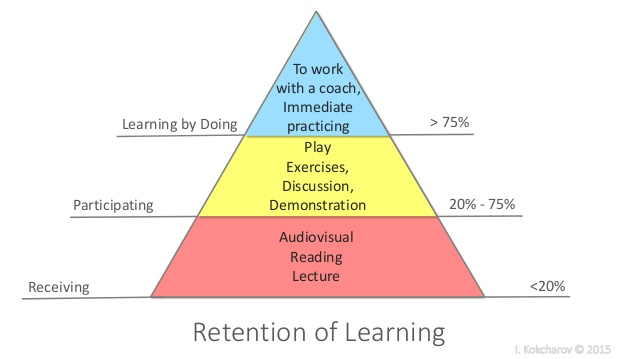
\includegraphics[width=0.9\linewidth]{figure/Analysis/skillslearn}
	\caption{Retention of Learning, taken from  \href{https://www.slideshare.net/igorkokcharov/kokcharov-skillpyramid2015}{\color{blue}here}}
	\label{fig:activelearn}
\end{figure}
\todo{Instead of "here" in the caption, we need to add a name, author, webpage or something}
\todo{Also, write caption that describes figure, don't do this in the above text.}

\subsection*{Passive Learning}
Passive learning is teacher-based where the students are not getting involved in the lecture. This form of teaching is usually seen on universities where the professors gives a lecture, and does not provide assignments or feedback to the students. This means that the learning method belongs in the bottom bracket of the retention of learning triangle as seen above. This way of teaching is usually the least efficient when the goal is to teach or alter information\cite{learning}.\\
\\
\subsection*{Sub Conclusion}
When learning is the goal in an education environment, both active learning and passive learning are being utilized. Based on the findings, active learning will provide a better learning experience where the student will be able to remember more information if done correctly. This means that participation and practice as well as motivation and interaction are essential to optimize the learning experience the most.
\todo{ville nok være smart at vi byttede rundt på de næste sektioner så en af de hernævnte emner kommer først. Dertil må vi huske at give en grund til at undersøge collaborativ learning (hænger det sammen med motivation eller hvorfor startede vi med at kigge på det i første omgang ? )}

\subsection{Collaborative learning}\label{collabLearning}

Seen through a biological perspective, humans are social animals\cite{laeringIPraksis}. This has a high influence on the process of learning, since humans as pack animals learn with and from each other - meaning that the learning process is social\cite{laeringIPraksis}. Working in groups and/or teaching each other, therefore strongly appeals to the human brain, and can be considered a powerful impacter when learning\cite{laeringIPraksis}.        

There has been a lot of research on collaborative learning in various educational contexts. However, the more artistic educations have been slightly overlooked\cite{collaborativeLearningTeachers}\cite{collaborativeMusicAnalysis}\cite{collaborativeLearningReview}. 
The article \textit{The Experiences of Elementary Music Teachers in a Collaborative Teacher Study Group} states, based on research outside of a musical context, that:\\
\begin{quote}
	\textit{"collaboration can improve learning outcomes if students make a conscious effort to coordinate their efforts and are able to come to a shared conceptual understanding of the problem being solved"}\cite{collaborativeLearningTeachers}.\\
\end{quote}
However, it is not an entirely unexplored area, and studies have shown that musical collaboration stimulates students critical and creative thinking, and rich musical experiences can surface from combining ideas from larger groups are combined\cite{collaborativeLearningTeachers}. 
The article introduces three principles of collaboration, that are based on interviews with three teachers:\\
\begin{enumerate}
	\item Collaboration facilitates student self-expression and independence.
	\item Students who are collaborating share goals. The teacher allows space for or guides students in creating productive student-student interactions.
	\item A teacher collaborating with her students facilitates their movement toward a shared goal. Teacher provides necessary background skills, creates student buy-in for the goal, and then fades away to allow students to take ownership.\\
\end{enumerate}
The first principle is at work when students, for example, are divided into smaller groups, and find themselves focusing on a task that generates communication, arguments and discussions without the teachers involvement. They will show independence as they individually will try to convince others to reach the same conclusions.\\

The second principle is related to a student groups shared motivation while focusing on a shared goal, for example presenting their work for the entire class, and sharing the responsibility to reach that goal.\\

The third principle is a teacher-student collaboration that also can be present withing the classroom. Here the teacher will for example instruct the student with harmonies, rhythms, chord progressions etc. after which the teacher gradually removes him/herself and let the students take control over the task at hand.\\


\subsection*{Sub conclusion}
Collaborative learning lies in the human nature and can be considered a great and positive influence in the learning process. Furthermore, is has an impact on various aspects of personal development such as creativity, musical influence and social interactions that could potentially be very useful later in life.


\subsection{Interaction in a learning perspective}\label{sec:interaction} \todo{cite for pokker da også! Jeg ved i kan :D !}
As mentioned in \autoref{sec:learning} a hands-on approach and interaction is important to get an efficient learning experience. This chapter will focus and go in depth \todo{with?} interaction in correlation to learning.\\
\\
First of, interaction is the description of the occurrence when objects or people interact with each other, this can be a person interacting with an object, or an object interacting with another object etc.\\
\\
As mentioned, it is important that the students and the teachers are actively involved in the learning activities to achieve as much as possible from their learning experience. First, students should have an opportunity to interact with teachers as well as the other students, to increase their learning opportunities. Secondly, the teacher should provide a classroom with room for involvement and motivation in the learning process\cite{interactionlearning}.\\
\\
A different view of interaction in a learning perspective is not only the interaction between students and teachers, but also a hands on approach for the students when learning about new subjects. This is also referred to as Kinesthetic learning or tactile learning. Kinesthetic learning is what describes a student carrying out physical activities rather than rather than \todo{gentagelse skal væk :)} listening passively to a lecture. This learning by doing approach is among the most popular learning methods among the students. This method gives the students space to experiment with trial and error as well as learn from their mistakes.\cite{kinest} \\
\\
As mentioned, many people will learn more with kinesthetic learning where movement and hands on using more senses will improve their learning outcome and learning experience\todo{det er der da ikke blevet sagt - ikke skriv "as meantioned når der slet ikke er blevet nævnt movement}. The amount of movement used in kinesthetic learning can depend on the assignment as well as the learning goal and can also vary depending on the amount of movement that is incorporated in the exercise\\

\subsection*{Sub Conclusion}
To improve the learning experience and the learning outcome, it is important to incorporate interaction in the studies. Giving the students the opportunity to interact with a subject which they are learning about, will increase their chance of remembering information and give them an easier time to learn it. Interaction can extend to incorporating more movement and is not excluded to hands-on approaches. More movement like running, jumping and dancing can also be included to increase the learning experience. \todo{ret underligt at have en konklusion på movement når afsnittet først kommer efter}\\
\begin{comment}
{\color{red}When trying to understand music in an interactive sense, one might look at another medium that incorporates interactivity: video games. In particular, one could look at interactive video games that focuses on playing or teaching music. Lily Gower and Janet McDowall conducted a study, in 2012, centered around the educational qualities gained from playing such interactive music video games\cite{interactiveMusicVideoGames}. The study aimed to establish if interactive music video games had an educational value when integrated into the existing music education.\\

The different games mentioned in the study were Guitar hero (See \autoref{sec:guitarHero}), SingStar and Wii Music. What these games have in common is that they all use interactivity as a means to playing music, be it with a guitar shaped controller, a microphone or the Wii remote held like an instrument. These games try to emulate what it would \textit{feel like} to play a guitar, sing or play different instruments.\\

The study interviewed two music teachers of different musical abilities, and 9 music students aged 11-14 (5 male and 4 female) from different socio-economic situations. The student participants came into the study with different levels of musical experience. The interviews were semi-structured of nature to allow free flowing conversation. Interviews with the children participants revolved around their prior music backgrounds and past experiences with interactive music video games. The interviews with the teacher participants discussed their personal views and experiences with interactive music video games, like Guitar hero (\autoref{sec:guitarHero}), in relation to music education.\\

Teacher two said during the interview that:
\begin{quote}
	\textit{"...the whole debate about whether it’s music making, that’s a whole other debate, but whether it’s developing some across the board generic skills, I’d say yes."}\cite[p.~98]{interactiveMusicVideoGames}.\\
\end{quote}
Meaning a belief in interactive music video games giving the students some educational values in a more general music setting. In addition, when asked about coordination benefits, Teacher two said the following:
\begin{quote}
	\textit{"...To play at the higher levels of that game [Guitar Hero] requires very high level coordination skills and you’re coordinating visually with what you’re playing as an instrument. So it’s not so different I think physiologically from what a musician does anyway which is to respond to a conductor visually, respond to the music score visually, and then play accordingly to a set tempo, and timing is everything. So, the game is about scoring high scores all based on your capacity to play in time on the right note and what’s that sound like? Sounds like music playing to me."}\cite[p.~98]{interactiveMusicVideoGames}.\\
\end{quote}
Teacher two has a firm belief that Guitar hero specifically has a high coordination requirement, and thus to play at the higher difficulty levels of the game, you need good eye-hand coordination, which he thinks correlates in a physiological way directly to the way real music is played.\\

When the student participants where asked about their musical knowledge gained from playing interactive music video games, one girl said:
\begin{quote}
	\textit{"Yeah, so it’s like you find out about more songs that you don’t know about . . . there’s a lot of songs that you don’t know about and then you like listen to them and then you get into either like the artist or the type of songs or you just listen to that song and stuff and then you go looking on the net for other songs of that type and stuff, so it opens up a whole lot of stuff."}\cite[p.~100]{interactiveMusicVideoGames}.\\
\end{quote}	
The participant felt that she had gained music knowledge, and broadened her musical identity. The exposure to the new music, gave her an interest in new artists and genres she might not have known about.\\

The discussion about whether or not interactive music video games provide the children with a basic understanding of essential musical elements, is argued by Lily Gower and Janet McDowalls, to be that they at least learned about pitch and rhythm, while maybe not the rest of the five elements seen in \autoref{list:basicMusic}. Meaning the interactive music video games assisted the children in Lily Gower and Janet McDowall's study develop some basic music skills, that might correlate to real music making\cite[p.~99]{interactiveMusicVideoGames}, and potentially could assist other children in similar age groups.

\subsubsection*{Sub conclusion}
In conclusion, the children in the study\cite{interactiveMusicVideoGames} did seem to learn at least two basic musical elements from interactive music video games, being pitch and rhythm. In addition the children also felt they had gained musical knowledge from these games. Hence interactivity in musical education, it being from Guitar Hero, SingStar or another interactive music medium, seems to assist children in development of some aspects of musical abilities.
}\todo{This part is not "Officially" part of interaction but still seems relevant, read through the chapter and see if it fits somewhere else}
\end{comment}
\subsection{Movement in a learning perspective} \todo{det virker fjollet at have dette lille afsnit når movement alligevel bliver snakket om ovenover? hvorfor er dette afsnit ikke bare inde under forrige? (specielt når movement bliver konkluderet på i tidligere afsnits konklusion)}
	In the book \textit{The Kinesthetic Classroom: Teaching and Learning Through Movement}\cite{kinestheticMovement}, it is argued that movement induces cognition, an argument that is supported by Dr. John Ratey in\cite{rateySpark}. Ratey argues that exercise before having classes improves focus and mood for students\cite[p.~33]{rateySpark}. This relates to active learning seen in \autoref{sec:activeLearning}, and kinesthetic learning in \autoref{sec:interaction}, as both relate to either being active or being physical doing learning.
\subsection{Motivation}
Motivation is an integral part to learning\cite{motivationGameDesign}, and is therefore important when looking at ways to assist children in learning music. The most fundamental motivational theory is the one called Self determination theory (SDT)\cite{SDT}. SDT proposes that motivation is divided into two brackets; Intrinsic motivation and extrinsic motivation\cite{SDT}. 

\subsubsection*{Intrinsic motivation}
Intrinsic motivation is the internal motivation, that pushes humans to do actions not depending on a specific reward, but wholly depending on the inner need to do the action, for the sake of it\cite{SDT}.
This is the inherent need humans have to learn, explore and widen their knowledge\cite{SDT}.\\

To establish what influences intrinsic motivation, the researchers behind SDT\cite{SDT} created Cognitive evaluation theory(CET) as a sub-theory within the existing SDT. CET is the theory that focuses on competence and autonomy in relation to intrinsic motivation. The first part of the theory says that social-contextual events that contribute to the feeling of competence for a performed action, improve the feeling of intrinsic motivation in relation to that action\cite[p.~70]{SDT}. These social-contextual events might include rewards, feedback and communications\cite[p.~70]{SDT}. For intrinsic motivation to be improved, the action that is performed must be accompanied by a feeling of autonomy\cite[p.~70]{SDT}.

\subsubsection*{Extrinsic motivation}
Extrinsic motivation is the motivation that drives a person, depending on a reward associated with the performed action. From the SDT theory extrinsic motivation is defined as: 
\begin{quote}
	\textit{The term extrinsic motivation refers to the performance of an activity in order to attain some separable outcome and, thus}\cite[p.~71]{SDT}.\\
\end{quote}
An extrinsically motivated action could be; performing a non enjoyable job, meaning that there is no intrinsic motivation to the work, but when a paycheck is introduced, the action would be extrinsically motivated.

\subsubsection*{Emotions}
Emotions and motivation have a sort of bidirectional relationship in which each side can activate or deactivate the other\cite[p.~66]{emotionsAndMotivation}. In addition to that, emotions directly impact the quality of learning\cite[p.~66]{emotionsAndMotivation}. In the book \textit{"Emotions and Motivation in Learning and Performance"}\cite{emotionsAndMotivation}, they use an example with a student named Jake, he has had past negative experiences with studying. This later deactivated his motivation to study in the future, because the negative emotions relating to the bad experience interrupted his goal of studying\cite[p.~67]{emotionsAndMotivation}. To better counter the negative emotions, and deactivation of motivation, one must consider highlighting the intrinsic task value of an action\cite[p.68]{emotionsAndMotivation}.
\todo{måske det burde nævnes lidt tydeligere hvor vigtigt positive følelser har? (måske enda kort i forhold til dopamin ?)}
\subsubsection*{Sub conclusion}
In conclusion, whether motivation is extrinsic or intrinsic, it is a core part of performing any action. Thinking about learning specifically, the intrinsic task value should be considered to be highlighted, so as to counter negative emotions.\todo{Put more weight on positive/negative emotions, in terms of motivation.}

\section{How is music taught? The Study plan} 
\todo{ måske vi skulle lave en blødre overgang mellem de to overemner? }
\todo{husk at udfylde citaternes placeholder}
According to the study plan, found on the website of the Danish Ministry of Education(Site) the children are required to learn three areas of competence. Within\todo{within - refererer til at der er flere, så der burde bare stå "these are"} these are musical performance, musical creation and musical understanding.

\subsection*{Musical performance}
Musical performance includes teachings about singing, movement and playing instruments. More specifically teaching the children about how to sing individually and in groups, as well as teaching them about different kinds of singing and songs. Furthermore, teaching the children about movement in a musical context, such as dancing and rhythmic movement. Finally, being able to play the basics of different instruments, such as drums, guitar, piano or keyboard and different wind instruments.

\subsection*{Musical Creation}
Musical creation includes the teachings of different abilities in relation to create, alternate or improvise musical pieces. The children should be able to compose music with the ability to remember time and tempo when creating music. Furthermore, the children should be able to form and shape sound into something rhythmic. Besides creating music, the children should also be able to change music with the help of adding sounds, or changing the pitch or pace of sound. Finally, the children should be able to improvise music without being given a specific assignment to follow.

\subsection*{Musical Understanding}
Musical understanding is, first of, to be able to express music in other forms than sound. For an example, they should be able to express themselves verbally about music and be able to draw music. The children should have knowledge about instruments, and the ability to distinguish the different instruments from their appearance as well as their sound. The children should be able recognize specific elements in a musical piece and identify them. Finally, they should have the knowledge of musical history, in relation to different music genres as well as music from different time periods.
\\

When the children get older \todo{"older" - hvor gamle snakker vi om, og hvor gamle er de børn vi snakker om nu da? det mangler der at stå}, they will be introduced to digital tools and synthesizers to be used in the classroom. These tools might include iPad or Garageband. On these devices, they are asked to compose a musical piece using the aforementioned knowledge.\\
In the lower grades \todo{igen hvilek klassetrin snakker vi om}, the children are working more with analog instruments as well as singing to develop a musical foundation for their education.
\\

The study plan opens for a broad interpretation of elements that are taught and with which tools this knowledge gets taught. After analyzing the study plan, it became evident that an interview with a teacher is necessary to get a profound understanding of how the course “Music” is taught in elementary schools.\\

\section{Problem Area}
As this report will try to improve current tools in modern musical education, it is important to understand how the current education functions. In order to establish a target group, the current musical education in elementary schools will be analyzed. Firstly, an interview with a music teacher at an elementary school will be conducted, to clarify \todo{possible} issues with the current education. \\	



\subsection{Interview with Hanna Jørgensen} \todo{kom i tanker om, har vi overhoved fået lov at at nævne hendes navn? }
Hanna Jørgensen is a teacher in music at both elementary school level and Danish Gymnasium level at Sankt Annæ Skole \todo{skriv at det altså er en mere speciel skole end en almindelig folkeskole}. She is also a pedagogue in Musical Pedagogy at the National Music Conservatory. Besides the aforementioned credentials, she is also involved in “Børne og Ungdoms Forvaltningen”, which is an organization that tries to improve the quality of life among children and young people \todo{undersøg nærmere, jeg husker det som værende specielt i forhold til skolesystemet, men det kan godt være at jeg tager fejl}. She is interviewed to help establish a detailed view on how the current musical education functions, and to help locate issues within the musical curriculum for elementary school children.
The interview with Hanna was conducted at Sankt Annæ Skole and was established to clarify how the current education functions in practice, and which issues are present in her opinion.\\ \todo{lidt en gentagelse af hvad der lige stod ? }

The beginning of the interview focusses on the current structure and tools used in the education. Hanna explains that the current study plan, for her class, is divided into clear courses with focuses on a particular subject. A few elements are consistent for the courses, in the way she teaches. Games and movement are two tools that are fundamental for how music is taught in elementary school. There are currently a set of tools used to teach music through games, she does however see a lack of general tools \todo{hvad menes der helt præcis her ? hvilke?}, and there is definite room for innovative ideas.\\

She also emphasizes the importance of Rhythm. Rhythm is a specific important thing that the children are taught. It is essential for singing, playing instruments and understanding music. This means that a focus is on the learning and understanding rhythm in elementary schools. The children mainly use singing as a tool for learning. Instruments are not used as commonly, as they are harder to get by and singing provides a tool that everyone possess, in order to learn rhythm. When it comes to the theoretical education, Hanna finds it essential to work with visual and physical tools. Currently \todo{nej, det var engang da hun underviste i USA. hun nævnte at hun savnede tæppet og måden at undervise med det} she uses a carpet with note lines drawn on it, as it is a physical tool and she can get the kids to collaborate when creating and understanding music. The collaboration is another theme, that Hanna finds important to teach the kids, however she finds a lack of tools currently. The class that Hanna teaches uses PC Software such as Garageband, but the interface is limited to a single user at a time. She is seeking physical tools that allows for creative thinking when collaborating. \\

Hanna is very clear, when she says that the children have an easier time learning, when working with physical objects. Another tool that Hanna uses in her class are Lego blocks \todo{nej så vidt jeg husker tegner hun dem kun. Hør interviewet igen}, which is a small tool that can be used in various ways \todo{at forklare hvad LEGO er virker lidt malplaceret, specielt da beskrivelsen ikke rigtig siger særlig meget alligevel}. She uses it to explain steps in music. She is very fond of the idea of physical blocks that can be used in versatile ways.
Hanna ends with the conclusion that the biggest issues she has currently, are physical tools that can be used collaboratively between her students.\\


\subsection{Workshop}\label{sec:workshop}
In order to get a closer look at the students learning music, a workshop was established at Sankt Annæ Skole. The workshop was created in collaboration with Hanna Jørgensen, who teaches a 4th grade class in music at Sankt Annæ Skole.\\

The workshop was conducted at Sankt Annæ Skole, which is not a regular public school. It does follow the general study plan of elementary school education, but it has a specific focus on musical education. Sankt Annæ Skole teaches musical concepts and performance on a higher level than a regular elementary school (Cite Sankt Annæ studyplan?). \\

The goal of the workshop was to get an idea of what the children thought about their current music education, what tools they use and how these tools could be improved. The children were presented with different ideas \todo{det skal uddybes meget havd der menes med ideer! vi havde jo lavet nogle mock-ups, og det skal også nævnes at disse var baseret på den daværende viden og derfor inden FPSen var færdig!}for new and alternative tools that can be used in the education. They had to provide feedback on the ideas and compare them to existing ideas, to find what elements of the different tools the students themselves desires.\\

Across the different ideas in the workshop, a number of themes became apparent. The following points were the most prominent when it came to desired features:\\


\begin{itemize}
	\item[-] \textbf{Movement}\\
	The students found the current education to be very still. They desired ways to be more active and have more movement as part of the education.\\
	\item[-] \textbf{Variation:}\\
	The students made it clear that they dislike using the same tools and same methods for learning various aspects. Having variation to keep things fresh would be more fun.\\
	\item[-] \textbf{Games:}\\
	The students love to learn through games. They feel like they remember a lot of what they learn, when they use games and they have fun while learning. \\
	\item[-] \textbf{Visuality:}\\
	The students asked for more visual components in their education. It is important to them that what they use are presented in front of them visually and had colors that were pleasing to look at.\\
	\item[-] \textbf{Physical:}\\
	The students, in extension of components being visual, loves when the tools are physical. If they can see, touch and feel the objects they use to learn, they have more fun and feel like they learn.\\
	\item[-] \textbf{Group work:}\\
	The students expressed great joy about working together with their classmates and collaborating in different ways about creating and understanding music.\\
	
\end{itemize}



\subsection{Target Group} \todo{jeg ville mene at det ville være smart at nævne at targetgroup også blev baseret på at vi har tilgang til dem gennem Hanna ( nu da vi også bygger en del viden op omkring netop dem gennem workshoppen. Dertil synes jeg virkelig der mangler at stå en sektion om at Sankt Annæ er en anderleders skole, og at vi gennem dette samarbejde må være opmærksomme på at de ikke nødvendigvis representere vores målgruppe helt så varieret som ønsket) }
Based on the knowledge gained about different learning theory, current tools used in education, an analysis of how the current education is and how the students perceive it, the target group will now be presented.
The target group for this project are children aged 8-12, currently residing in elementary school and participates in the course “Music”.\\

The findings display a great potential to provide a tool for these students.
Furthermore, the teachers of the course “Music” will be considered a sub target group for the project, as the tool this project aims to provide would have to be used and explained by the teacher. The teacher would have to use the tool to provide knowledge and add meaning to what the tool represents.
 
 
\subsection{Learning tools used}%Mini SOTA
This section is about the learning tools that the target group have been using in classrooms. It concentrates on music material used in schools and what Hanna from Sankt Annæ uses for helping her students understand music notation and music theory. It is important to note that Sankt Annæ is a school that uses music as their main learning objective.  

\subsubsection{Garage Band}
Garage band is a software developed by Apple, Inc. It is used for allowing users to create, editing and rendering music. The whole idea about Garage band is that the software uses pre-made MIDI keyboards, loops and arrays of different instrumental effects and voice recordings that can help the user further develop various sounds. This software is a very helpful tool for learning how to create music.\cite{Garageband}
\begin{figure}[H]
	\centering
	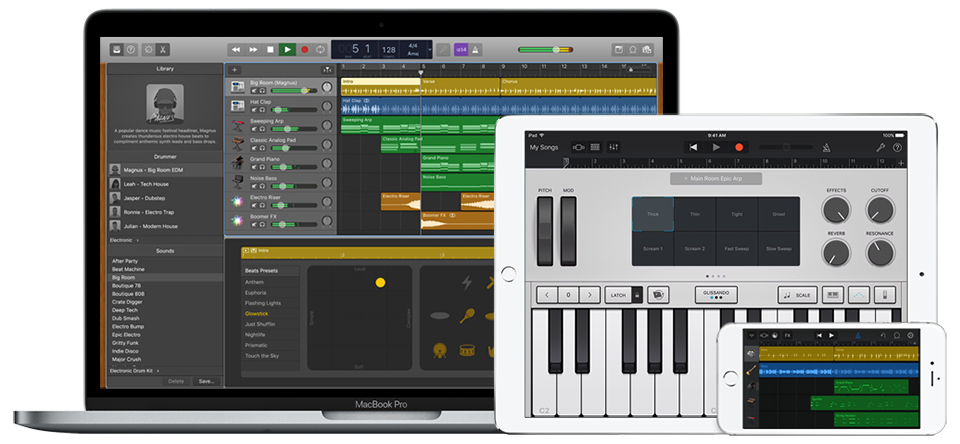
\includegraphics[width=0.7\linewidth]{figure/Analysis/garageband}
	\label{fig:garageband}
	\caption{Show Garage band is compatibly on tree different devices and what the software looks like \cite{GaragebandPicture}}
	
\end{figure}


\subsubsection{MuseScore}
MuseScore is an open-source software program for creating music notation. The main attraction of the software is the ability to play and practise sheet music anywhere. You are able to search for new music sheets and practice thsese by either listening to the notes or change the notation. It is available for windows, mac, IOS, Android and Kindle Fire. It has an input via MIDI keyboard and can transfer to and from other programs via MusicXML, MIDI etc. This is a very useful tool for understanding music notation and practice it hands on. This software is a good example on learning notation for beginners to expert or just experts that want to create music. The program is build so that anyone wanting to create music can. MuseScore also provides their own definite guide to MuseScore. In contrast to many other softwares that lets one build notation sheets, this specific software is free. \cite{MuseScore}

\begin{figure}[H]
	\centering
	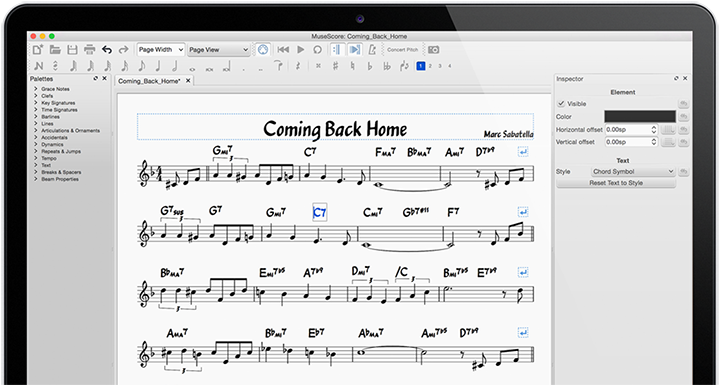
\includegraphics[width=0.8\linewidth]{figure/Analysis/musescore.png}
	\label{fig:MuseScore}
	\caption{shows a caption of a sheet music that can be played or manipulated to understand the music notation \cite{MuseScorePicture}}
\end{figure}

\subsubsection{Go Fish - Music notation} 
Go fish is a card game played by two or more players. The rules state that five to seven cards are given from a standard 52-card deck to each player. The remaining cards are spread out on a table. When it is a players turn, that player can ask any other players if they have the same card value (this means the same number value). If they do, that card is given to the player that asked and if they don’t the player is asked to “go fish” which means the player who asked has to pick a card from the pile of cards on the table. The idea for winning is then to gather as many sets of cards of the same value. This game can be used for many other purposes than using the standard game of go fish with a standard 52-card deck. Hanna from Sankt Annæ is playing this game with her students where she do not use the standard 52-card deck but uses cards with music notation. Making it a learning tool for people trying to memorize or learning the different notations of music. \cite{GoFish}

\begin{figure}[H]
	\centering
	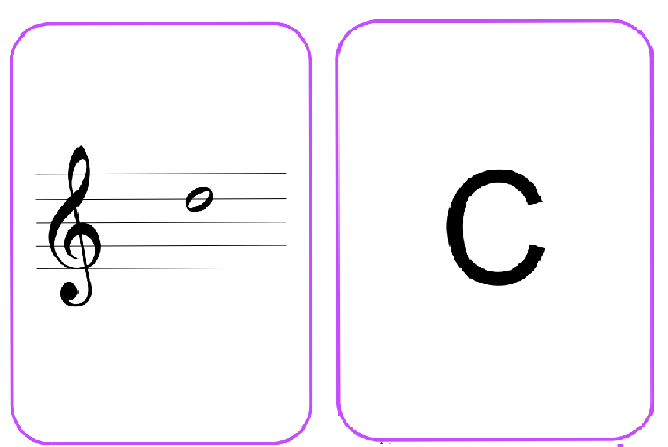
\includegraphics[width=0.7\linewidth]{figure/Analysis/gofish}
	\label{fig:gofish}
	\caption{An example taking from ... that shows how Go fish can be played with notes \cite{GoFishPicture}}
\end{figure}

\subsubsection{Sibelius}
Sibelius is a software program for creating music notation. It was created by Sibelius Software. The software can edit, print, play the music using synthesized sounds, produce scores and public scores for others via the internet. The software supports all music notation as well as the most complex notation to produce. It can be used for playing the music or turning it into MIDI or either audio files. It supports basically any MIDI device and it also comes with some pre-made sample files. It also uses third party plug ins such as Vienna Symphonic Library or Mark of the Unicorn’s symphonic instrument. \cite{Sibelius}

\begin{figure}[H]
	\centering
	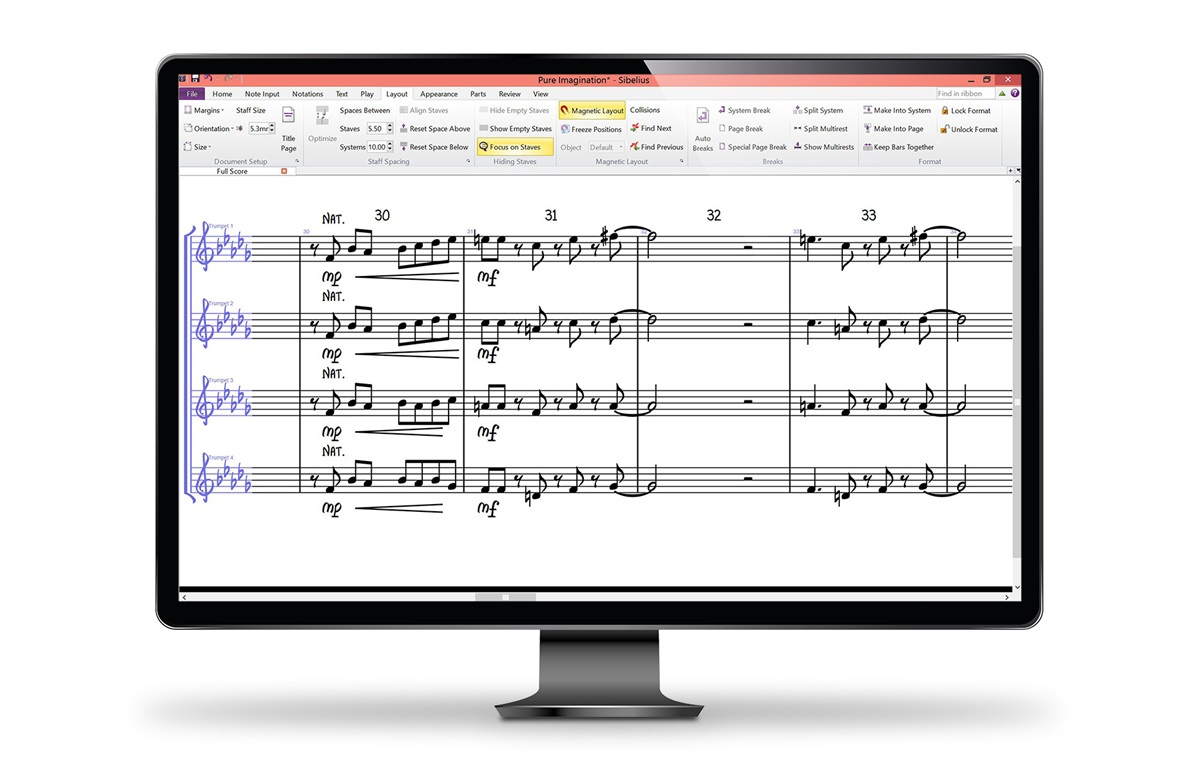
\includegraphics[width=0.7\linewidth]{figure/Analysis/Sibelius}
	\label{fig:sibelius}
	\caption{Shows what the software looks like with different notations \cite{SibeliusPicture}}
\end{figure}

\subsubsection{Clio Online} 
Clio Online is an online tool for students who wants to learn more about the different topic provided in high school. You can learn topics such as Danish, English, German, religion, history, biology, sports, music, arts, food etc. This is a tool used by teachers to help their students with their studies. In every subject there is help tools such as videos, sound files and pictures to optimize each induvials learning pattern. This online tool also provide the user the capability to choose what difficult level the material should be. \cite{ClioOnline}


\subsubsection{Music work out}
Music work out is a physical tool set developed by Anette Præst Nielsen. It is a box consisting of different games or teaching methods for users who want to learn or have fun with music. There are currently two different editions – A teacher’s edition and a Game edition.  The Teacher’s edition contains: Around 800 cards and accessories. It is used for learning about theory, notes- and ear training, rhythm cards, interval cards, rest cards, time signature cards, solmization cards, subdivision cards, clef card etc. The game edition contains: 3 different games – Domino, bingo and memory. Which also consist of different parts of the above topics. \cite{MusicWorkout}

\begin{figure}[H]
	\centering
	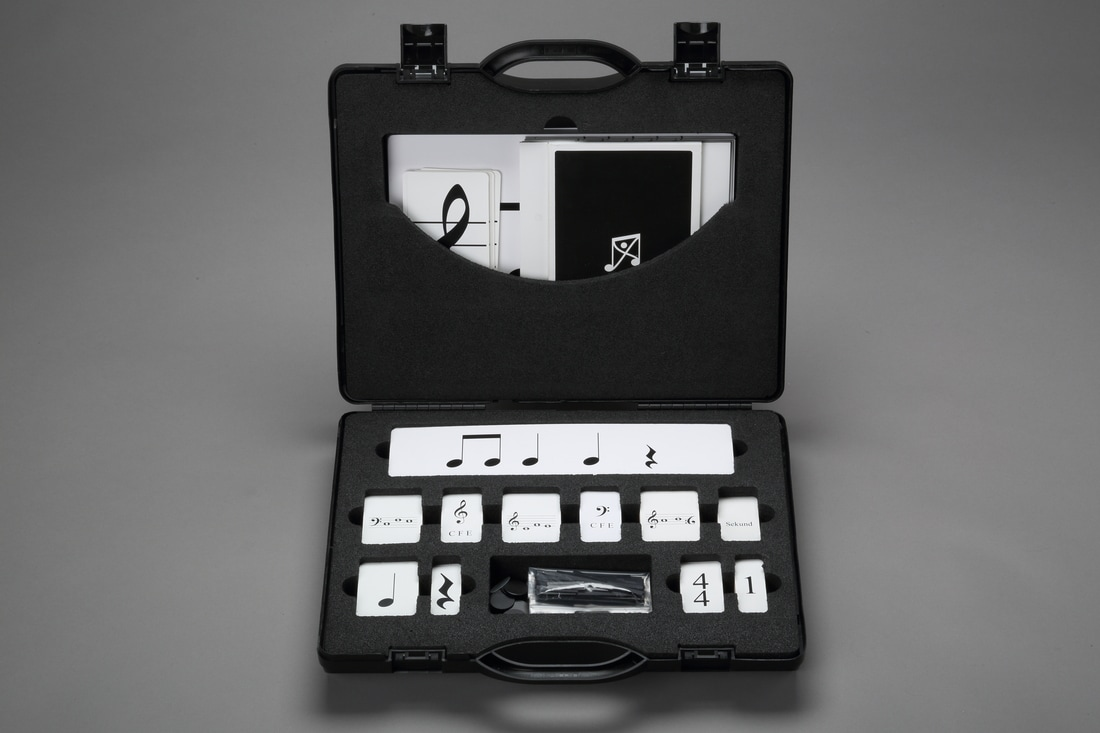
\includegraphics[width=0.7\linewidth]{figure/Analysis/musicworkout}
	\label{fig:musicworkout}
	\caption{An example of the teacher's edition for learning about music notation \cite{MusicWorkoutPicture}}
\end{figure}

\subsubsection{Music mind game}
Music mind game is developed by Michiko Yurko. It is physical games providing alphabet cards, blue jello sticks and bingo cards. The various subject areas that can be bought are dictation and sight signing, alphabet and intervals, reading rhythms, rhythm math, staff and notes, tempos, music symbols, scales and key signatures, triad and chords. All these games are great learning material for teaching children music. \cite{Musicmindgames}

  
\subsection{Choice of Direction}
The knowledge gained in the problem area chapter, provides a direction for the progress of the project. A look at the study plan gives an overview of how the schools currently teach music through the three areas of competence; Musical Creation, Musical Knowledge and Muiscal Performance. An elaborated interview with Hanna Jørgensen provides insight in current issues with the musical education, which leads to an analysis of the potential target group. This helps establish the target group of 8-12 years old.\\

With the target group established, an analysis of the tools currently used by the target group, in the context of the information gathered through the interview and workshop, highlights issues with a lack of physical tools that the target group can use to learn music in collaboration with each other. Both Hanna Jørgensen and the children asked in the workshop expressed issues with the lack of tools, that can be used when working in groups, while being a physical tool, that the students can touch and have visually presented in front of them.\\

With the knowledge gained in the initial analysis and regarding the study plan, the project will aim to focus on the aspects of musical creation \todo{nope det er ikke blevet besluttet :) }, as the workshop displayed that the target group expressed a need for new tools to learn elements of this specific area of competence.
The following analysis will focus on the aspects found in the problem area. Collaboration and how working in groups affect learning will be researched \todo{det er jo blevet forklaret hvordan det påvirker lærring, men nu bliver flere og mere i dybdegående forskellige aspekter diskuteret, herunder metoder til hvordan man kan samarbejde, og hilke fokuspunkter man bør være opmærksom på for at få det til at lykkes} , to gain a broader understanding of how a product could be developed, that fills the requirements of the target group.\\

\todo{jeg vil mene at det giver mening at indsætte FPS her da det er her vi specificere vores retning. }



\section{Working in groups - different aspects and approaches} % Sofie (sammenflet)

When working in groups different aspects affect the productivity and level of performance \cite{GodKlassekultur} and thereby affects the learning outcome for both the group and individuals. In this section some of these aspects will be discussed. These include: The arrangement of groups, the teachers role, roles within a group, inclusion and exclusion from a group, Feedback as an important group tool, and different collaborative learning Methods - Cooperative Learning, Constructive Competition, and Peer Learning.

\subsection{The arrangement of groups}\label{GroupArrangement}
Practical issues such as arranging tables in rows does not promote ideal group work but is more useful when a teacher is speaking to entire classes\cite{collaborationSocialPedagogy}. A more flexible table arrangement is more preferable, as it can be customized to fit the work process and group size\cite{collaborationSocialPedagogy}. 

The number and sizes of the groups need to be taken into account and correspond to the total number of students and teachers within the class. Assuming that there is a classroom with 32 students a grouping of 4 students in each group will mean that a teacher needs to prepare and manage 8 groups which can be more difficult. Fewer larger groups with more members, 6-8 pupils, however, will be more convenient for a teacher to manage, but the learning outcome of the individual students within the group might not be ideal\cite{collaborationSocialPedagogy}. The smaller the groups the better the cooperation and beneficial effects of competition can arise\cite{collaborationCompetitionGames}.

\subsection{The roles within a group}
Group stability and dynamics are other factors that teachers might need to consider. It might be more beneficial for the students to be arranged in groups based on the teachers prior knowledge about the students' behavior and stick to the same groups for longer periods\cite{collaborationSocialPedagogy}, as this gives the group time to challenge the knowledge in the group, and learn the members differences and thereby gain understanding of the importance of different work approaches and processes\cite{laeringIPraksis}.

Differences among people when working in groups are important, as the group members then contributes in different areas (both academically and social), and can thereby overlap each others strengths and weaknesses \cite{ProjektarbejdesKompleksitet}. These individual collaborative roles (based on Belbins team roles \cite{ProjektarbejdesKompleksitet}) can be categorized in three main categories: 
\begin{itemize}
	\item[-] The thinking role - focus is, being creative making ideas, and the outcome of the work. 
	\item[-] The doing role - the focus is the process of the work (how and why)
	\item[-] The social role - focus is the wellbeing of the group. 
\end{itemize}

Having a representative from each category strengthens the group work and outcome thereof - and thereby the learning outcome\cite{ProjektarbejdesKompleksitet}. However if not represented and/or the importance of each role is not acknowledged, it can led to conflicts within the group. These conflicts, can often be seen as difficulties within certain areas (eg. problems with organizing, leading to unstructured work), or the feeling (and expression) of a not equal contribution, which can lead to social conflicts (which in some cases leads to exclusion from the group)\cite{ProjektarbejdesKompleksitet}. 

\subsection{Social inclusion and exclusion}
Being a part of a community/group lies within human nature and is important for the individuals wellbeing  \cite{ProjektarbejdesKompleksitet}- thereby also their motivation, and can therefore effect the learning process. Being excluded from a group has a negative effect on the individuals learning and social wellbeing. This can even influence the person being excluded to avoid future group work due to the psychological defeat. The Danish professor in social psychology Dorte Marie Søndergaard, calls this \textit{social exclusion anxiety} \cite{ProjektarbejdesKompleksitet}. Being excluded is often related to the contributions (or lack of same) value. If the group members contribution does not meet the requirements or is seen as of less value, exclusion can occur. Exclusion can also be caused by character traits and personality, and might therefore not necessarily origin from academical reasons \cite{ProjektarbejdesKompleksitet}.
To reduce the risk of exclusion (and facilitate inclusion), the group must function socially and (as mentioned ) understand the importance of the different collaborative roles. The tasks that groups need to complete have to be designed in such a way that encourages collaboration and discussion and not promote individual work in order to produce an effective learning outcome \cite{collaborationSocialPedagogy}. To further enhance inclusion, the tool of Feedback can be used. 


\subsection{Feedback}
Feedback given between members of the group, is a highly important part of group work\cite{laeringIPraksis}\cite{ProjektarbejdesKompleksitet}. It is with this tool that the group can reflect on their work, and together work towards a joined goal, improving the learning process and outcome for both group and individuals\cite{laeringIPraksis}\cite{ProjektarbejdesKompleksitet}. It is also a tool which can be used to acknowledge each others work, and enhance inclusion and social wellbeing\cite{laeringIPraksis}\cite{ProjektarbejdesKompleksitet}. 


\subsection{Collaborative learning Methods} 
When collaborating, the process and methods must relate to the type of work/assignment. Collaboration can therefore be conducted in many ways. In the following sections three acknowledged collaborative methods, namely \textit{Cooperative Learning, Constructive Competition, and Peer Learning}, will be discussed.  

\subsubsection{Cooperative learning}
A term which is used widely within the umbrella term collaborative learning(see \autoref{collabLearning}) is cooperation\cite{collaborationCooperation}. It is a teaching strategy in which children in smaller groups in a class room cooperate towards a common goal and thereby develop their social skills whilst building a common base of knowledge about a course subject\cite{collaborativeLearningTeachers}\cite[p.~15]{peerLearning}\cite{collaborationCompetition}\cite{cooperativeLearningPractice}. A teacher divides the student into smaller groups for either a long or short term period and assigns a task for them. The students are, thereby, responsible of each others learning and cooperate towards the groups success in solving the task at hand. Meanwhile, the teacher walks around between groups and monitors their progress\cite{cooperativeLearningPractice}. Even though cooperative learning has shown positive results in learning outcomes of pupils, it has also been criticized For example because there in some cases will be students taking on most of the work, while others do nothing. It is also criticized for the risk of it causing competition between either group members or whole groups\cite{collaborationCooperation}.

\subsubsection{Constructive Competition}
Competition tends to be seen as a negative and destructive force when talked about in a learning context and is often conceptualized as an opposite to collaboration\cite{collaborationCompetition}. Humans compete to outshine others in various situations such as at work, in school or in games\cite{collaborationCompetitionGames}\cite{collaborationCompetition}. However, in the right conditions it can be constructive as it is simultaneously a strong motivator in learning situations\cite{collaborationCompetitionGames} and makes pupils stretch beyond their own expected abilities\cite{collaborationCompetition}. Competition is one of the core mechanics in video games and, aside from  motivation, it increases excitement, involvement, attention and if such a game is educational, these effects could potentially have positive effects on learning\cite{collaborationCompetitionGames}. 

\subsubsection{Peer Learning} %Sofie
In Peer Learning, equal individuals (eg two students) (non professional) work together (in peers) to archive their individual goals \cite{peerLearning} - often in a "tutor/mentor"-"tutee/mentee" relationship. The idea is, that through mutual help and support, knowledge should be shared between them, as so the goals will be to either learn by teaching or by being taught. This can be done in different constellations\cite{collaborationCompetition}.

\begin{description}
	\item[Peer Instruction] The students meets prepared in given subject, the teacher asks a question in the subject, and the individuals state their answers. Next, the assigned peers discuss the question and based on this, state their reevaluated answers. In this process the students have prepared themselves in the same material, and so their knowledge might not vary significantly, and the roles of tutor and tutee might not be present.  
	
	\item[Peer Tutoring] Each of the peers must prepare and be able to teach individual given material, to the other peer. The peers is therefore in the roles of \textit{Tutor} and \textit{Tutee}, and shifts roles after a certain amount of time. This process relies on the fact that each of the peers have a greater understanding in a subject than the other, as the roles of tutor and tutee will become present.     

	\item[Peer Mentoring] This resemble the process of Peer Tutoring, but instead the students must have different skill and experience level (eg. comes from two different grades). Instead of a tutor and tutee, the terms \textit{Mentor} and \textit{mentee} is often used, as the social relationship is often more in focus than achieving academically skills.      
\end{description}   

For all different approaches to Peer Learning it applies that, the teacher must have a deep understanding of the individual students, both in terms of social and professional skills \cite{collaborationCompetition}. Otherwise the Peers might not have the right prerequisites for the collaboration.
Furthermore as Peer learning revolves around the will to share knowledge, the Peers approach to the process is crucial for the success of the process\cite{collaborationCompetition}.


\subsection{Sub conclusion} %Sofie og Jens
Understanding how the teacher should (preferably) form groups, and how the dynamics of the group members affects the work, will help in understanding how the tool of this project should strive to relate and support both these arrangements and collaborative roles. The purpose of this focus should be inclusion, and thereby a higher learning outcome for both the group and for the individual. 
When having this focus, the collaborative methods can act as guidelines for the design and usage of the tool.\\

As most of the factors concerning group forming, dynamics, and arrangements,  will be in the hands of the teachers, they might not be something that can be directly designed for.  
However, based on the section's findings, it was found most suitable, if the tool could be used for groups of the size 2-6 students and should rely on a flexible seating arrangement.
 

\section{The classroom environment -understanding the context} %Jens
\todo{must be written}


The fact that children spends a large amount of time in a class room, means that the environment of the class room itself has a significant impact on the students’ education. There are numerous ways of affecting the students in a positive way through physical elements, such as the placements of the students’ desk or the type of wall art decorating the classroom.\cite{classroomsetting} The following section will investigate which aspects of the class room setting are important to keep in mind, when designing a product for an elementary school class.\\

\subsection{Seating}
The placement of the students is a main concern when discussing a classroom setting. There are pros and cons of different setups that affect how teaching occurs.
The most commonly used setup, is rows of tables pointing towards a fixed point with the teacher in focus. This setup is ideal for students to focus on their own work, but significantly limits the interaction that children has with each other and the teacher.\cite{classroomsetting} \\

An alternative approach is to have the students sit in larger groups. This approach highlights interaction for the individual student. It is ideal to use if students collaborate with each other about projects but runs the risk of increased disturbance and a higher amount of background noise.\cite{classroomsetting}\\

The final approach for the organization of students, is a setup where all students are placed in a circle or square, around the classroom. This setup ensures that all students are at an equal distance to the point of focus, ie., the teacher, and that everyone would feel equal and part of a larger team.\cite{classroomsetting}\\

\subsection{Decoration}
How the room is decorated is an important consideration in the classroom setting. It is important to have a balance between colorful artwork, such as drawings, or colored note boards and school related information, such as deadlines, expectations of the students etc.\cite{classroomsetting} It is important to find the right balance for the individual class. If the classroom is too organized it risks stifling creativity. If the classroom does not have enough organization, it risks that students lose focus and gets distracted easily.\cite{classroomsetting}\\

\subsection{Noise}
The final concept investigated in terms of classroom setting, is the noise of the classroom. There is evidence that too much noise interferes with the students’ ability to understand and process what is presented to them.\cite{classroomnoise} If a classroom is affected to a consistent high amount of background noise, it can result in a worsen understanding of speech.\cite{classroomnoise} The specific parts of the classroom that are important to consider when it comes to background noise, are air conditioning and heaters or other electronical equipment, and how the surface of the physical classroom reflects noise.\cite{classroomnoise}\\



\section{State of the art - Design Inspiration}\label{sec:sota}
In this section of State of the art the focus will be on the design inspiration conducted from the analysis. This will be the inspiration for development design requirements and design. It will provide aspect from physical interfaces to digital interfaces. In the end a sub conclusion will be represented to gather all the main points from State of the art. 

\subsection{Guitar hero}\label{sec:guitarHero} 
Guitar Hero is a game developed for playing games while using low profile MIDI components that resembles instruments. The game was developed by Harmonix. The first Guitar Hero gamee uses a guitar shaped controller that enables the player to feel the imitation of playing rock music. The whole idea is that the player will see notes on the screen in different colors, and each color is also resembled on the guitar. The idea is then for the player to match and press the correct color coding. Other features that have been added are moving the guitar while pressing the long analog that resembles the guitar strings. 

The features used in Guitar Hero such as color coding combined with movement while still learning about patterns can be reused again in a many other aspects of user centered design or a user centered interface. Considering that the target group in this report does not need to learn anything specific but still making a tool that can optimize a learning pattern, Guitar Hero provides a consistent learning pattern. It provides the user the capability of choosing the song and what level each song should be played on. \cite{GuitarHero}
 
\begin{figure}[H]
	\centering
	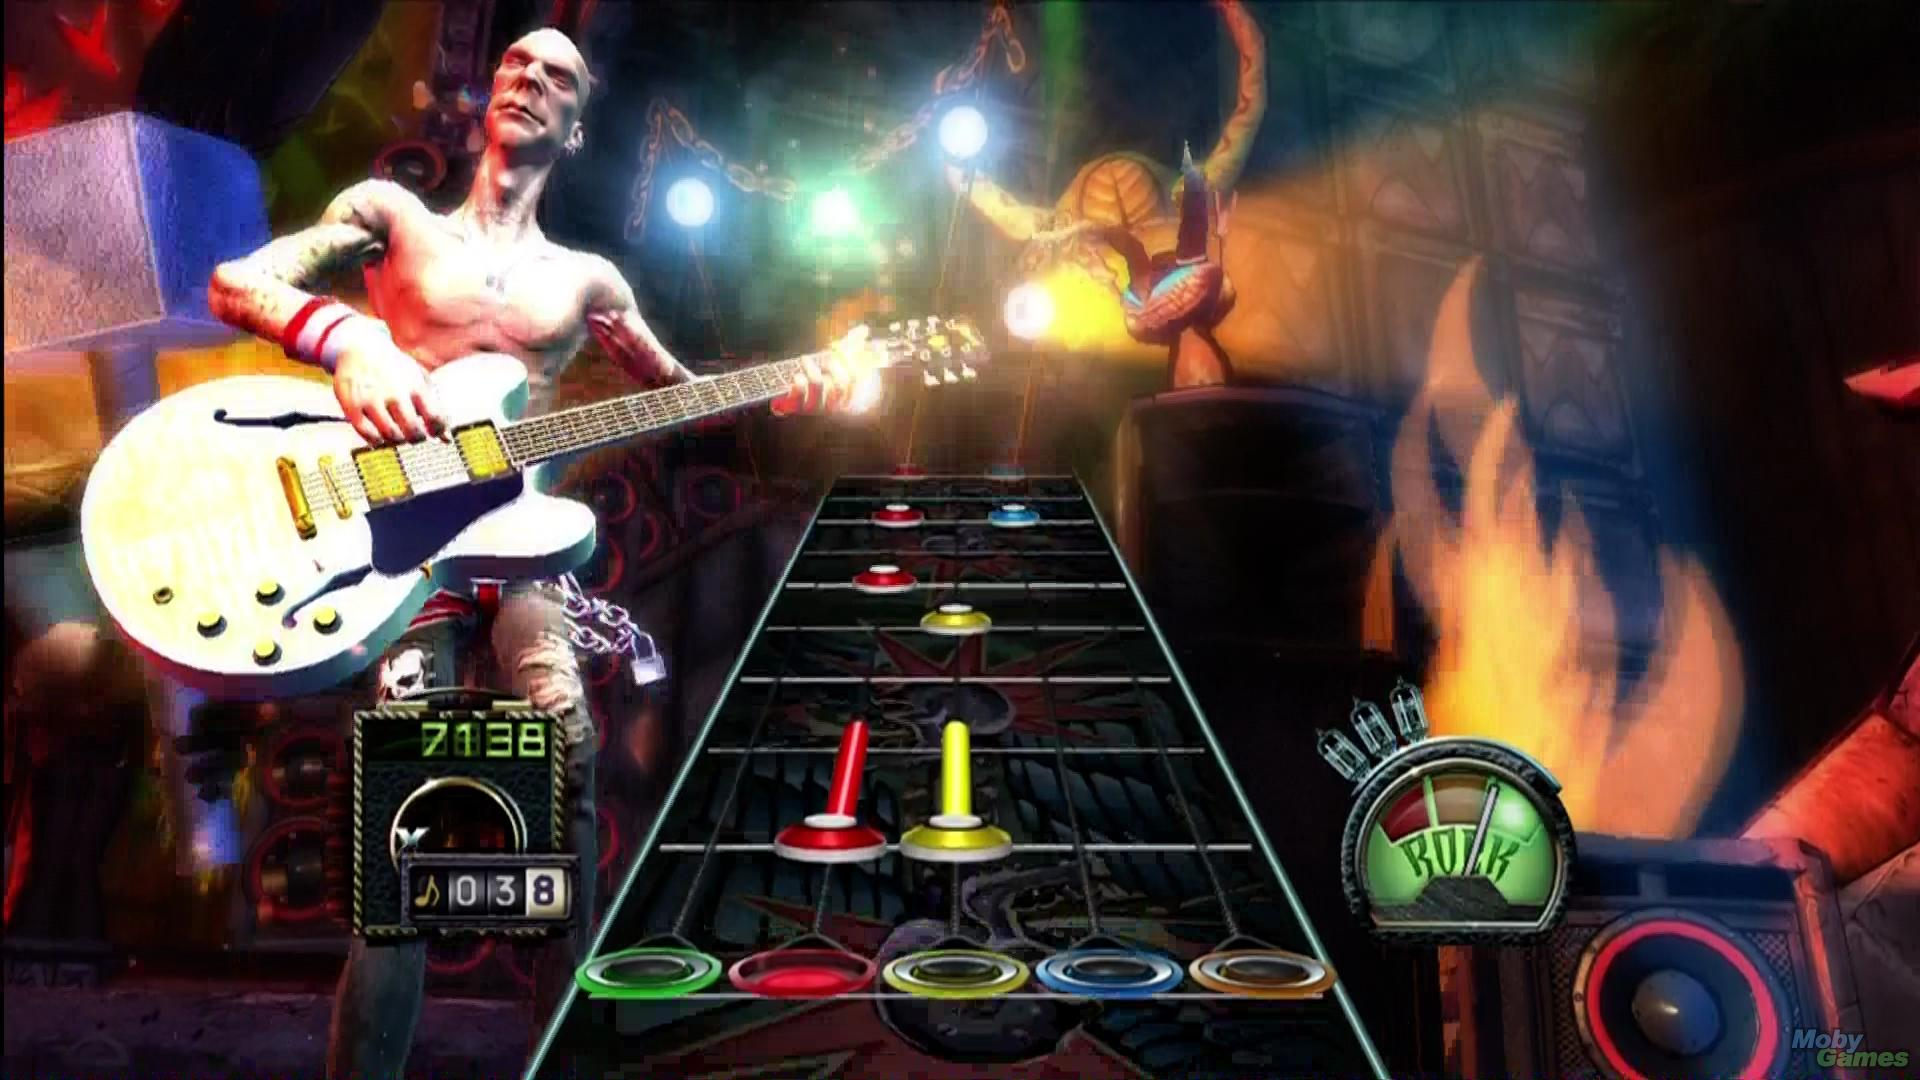
\includegraphics[width=0.7\linewidth]{figure/Analysis/guitarhero}
	\caption{Screen shot of a user playing Guitar Hero showing how it looks like on screen \cite{GuitarHeroPicture}}
	\label{fig:guitarHero}
\end{figure}



\subsection{Noteput} 
Noteput is an interactive music table with tangible notes. It is made for learning notation. The idea is that you use the interactive screen that shows a staff which can be either a Treble Clef or Bass Clef, thereafter you can choose between the different notations and place them on the staff to determined if they should be whole, half, quarter, eights, sharp, flat or natural notes. The table also has an option to play the music or loop the music so the user can keep changing the sounds as the loop keeps playing. 

Since this report is targeting children aged 8-12, this interface could make the learning experience much more interactive. During the workshop is was established that the children wanted more movement, variation, gamification, visuality and physical which makes Noteput a definite inspiration for further development. The important parts of Nopteput is the physical and tactile interface. \cite{Noteput} 
\begin{figure}[H]
	\centering
	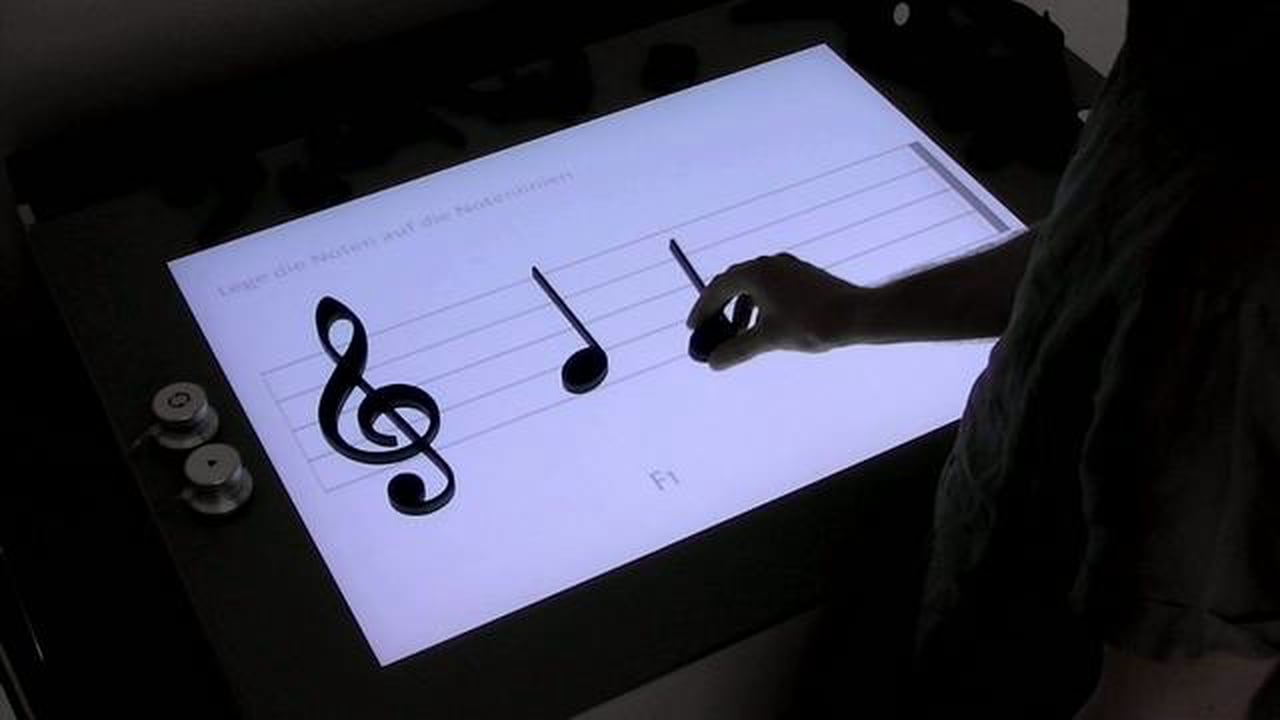
\includegraphics[width=0.7\linewidth]{figure/Analysis/noteput}
	\label{fig:noteput}
	\caption{Shows the idea behind placing tangible notes on the ineractive screen \cite{NoteputPicture}}
\end{figure}
\todo{cite + Guitar Hero med store bogstaver, gerne i italic.}


\subsection{Dato duo} 
Two person synthesizer for kids, no apparent learning outcome, but seems fun to play around with. Dato duo is a combination of a synthesizer and sequencer for creating electronic music together with people. It can be played alone or with others. It is meant to target children and adults interested in making music. On one side it is build using the circular sequencer which is a loop that loops the last eight notes that is played and playing a melody into it using the pentatonic keyboard (for example like using the black keys on a piano). On the other side are the controls for the synthesizer which contains two sliders that controls the two digital oscillators and the filter-cutoff frequency. It can also be combined with MIDI components and a sync input and output. 

This physical tool is showing how to corroborate sounds together. It can be played alone but the optimal part is playing it together with other people. This device focus on giving each user different component to control and this is the important factor of this device. Each component helps the users combine and make the device much more collaborative in making sounds together. \cite{Datoduo}
\begin{figure}[H]
	\centering
	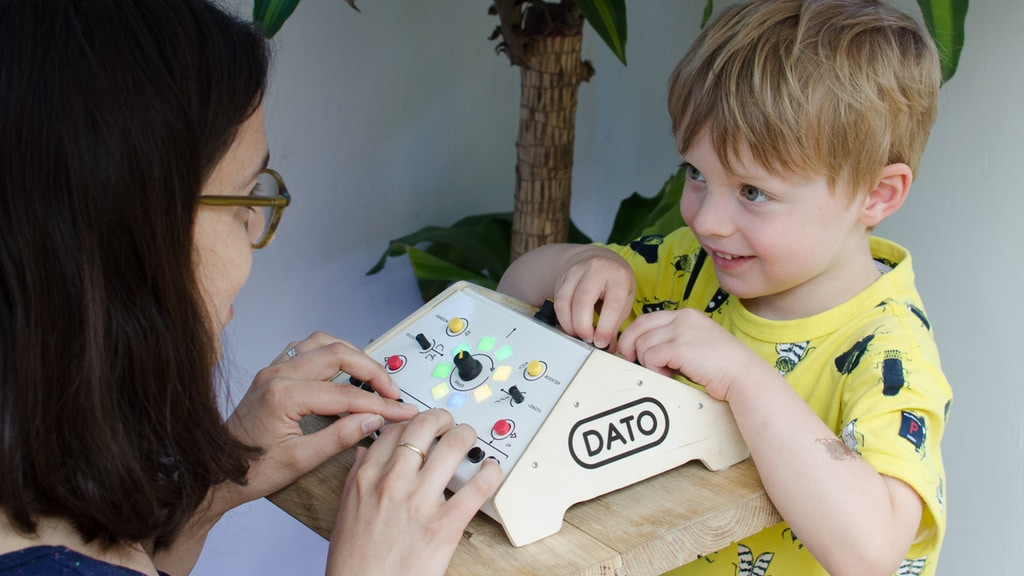
\includegraphics[width=0.7\linewidth]{figure/Analysis/datoduo}
	\label{fig:datoduo}
	\caption{Shows the Dato duo synthesizer being interactet with by two users \cite{DatoduoPictures}}
\end{figure}

\subsection{Drop mix}
Dropmix is a hardware instrument for creating, freestyling, competitive or partying with music. It uses a large board with 5 different slots for placing cards of different values. It is operated by using a phone or tablet for playing each different mode which are clash, party and freestyle. Clash mode is a competitive game for 2 to 4 players. The goals of the game is to be the first team to reach 21 points. Each card that is placed on the table scores a point. To replace a card in one of the slots, it must be either equal or a higher level than the card already in the slot. Each card has to be placed into matching colored slots. There are also multicolored wildcards and black and white effect cards that can be placed onto any of the 5 slots. In party mode all players play together to play cards for mixing music and score points. The goal is to get the high score the crowds request as fast as you can. Request will then appear on the screen for a limited amount of time. Request can be for cards with certain level, color or instrument. Freestyle mode is all about mixing the different cards to create various beats. When you see the DM icon press the Dropmix button to spin the equalizer if the equalizer lands on the level then remove all the cards from that spot equal to the cards of that level. If it lands on the X clear all slots. The faster you meet each request the more points you will earn. 

Drop mix is a combination of collaboration and a physical interactive installation. This physical tool uses tree different kinds of play modes and it could be develop even further for school usage. The importance of the device is the capability to change between playing together or against one another. It uses a board and cards which makes this playable anywhere since it does not take up very much space. \cite{Dropmix}

\begin{figure}[H]
	\centering
	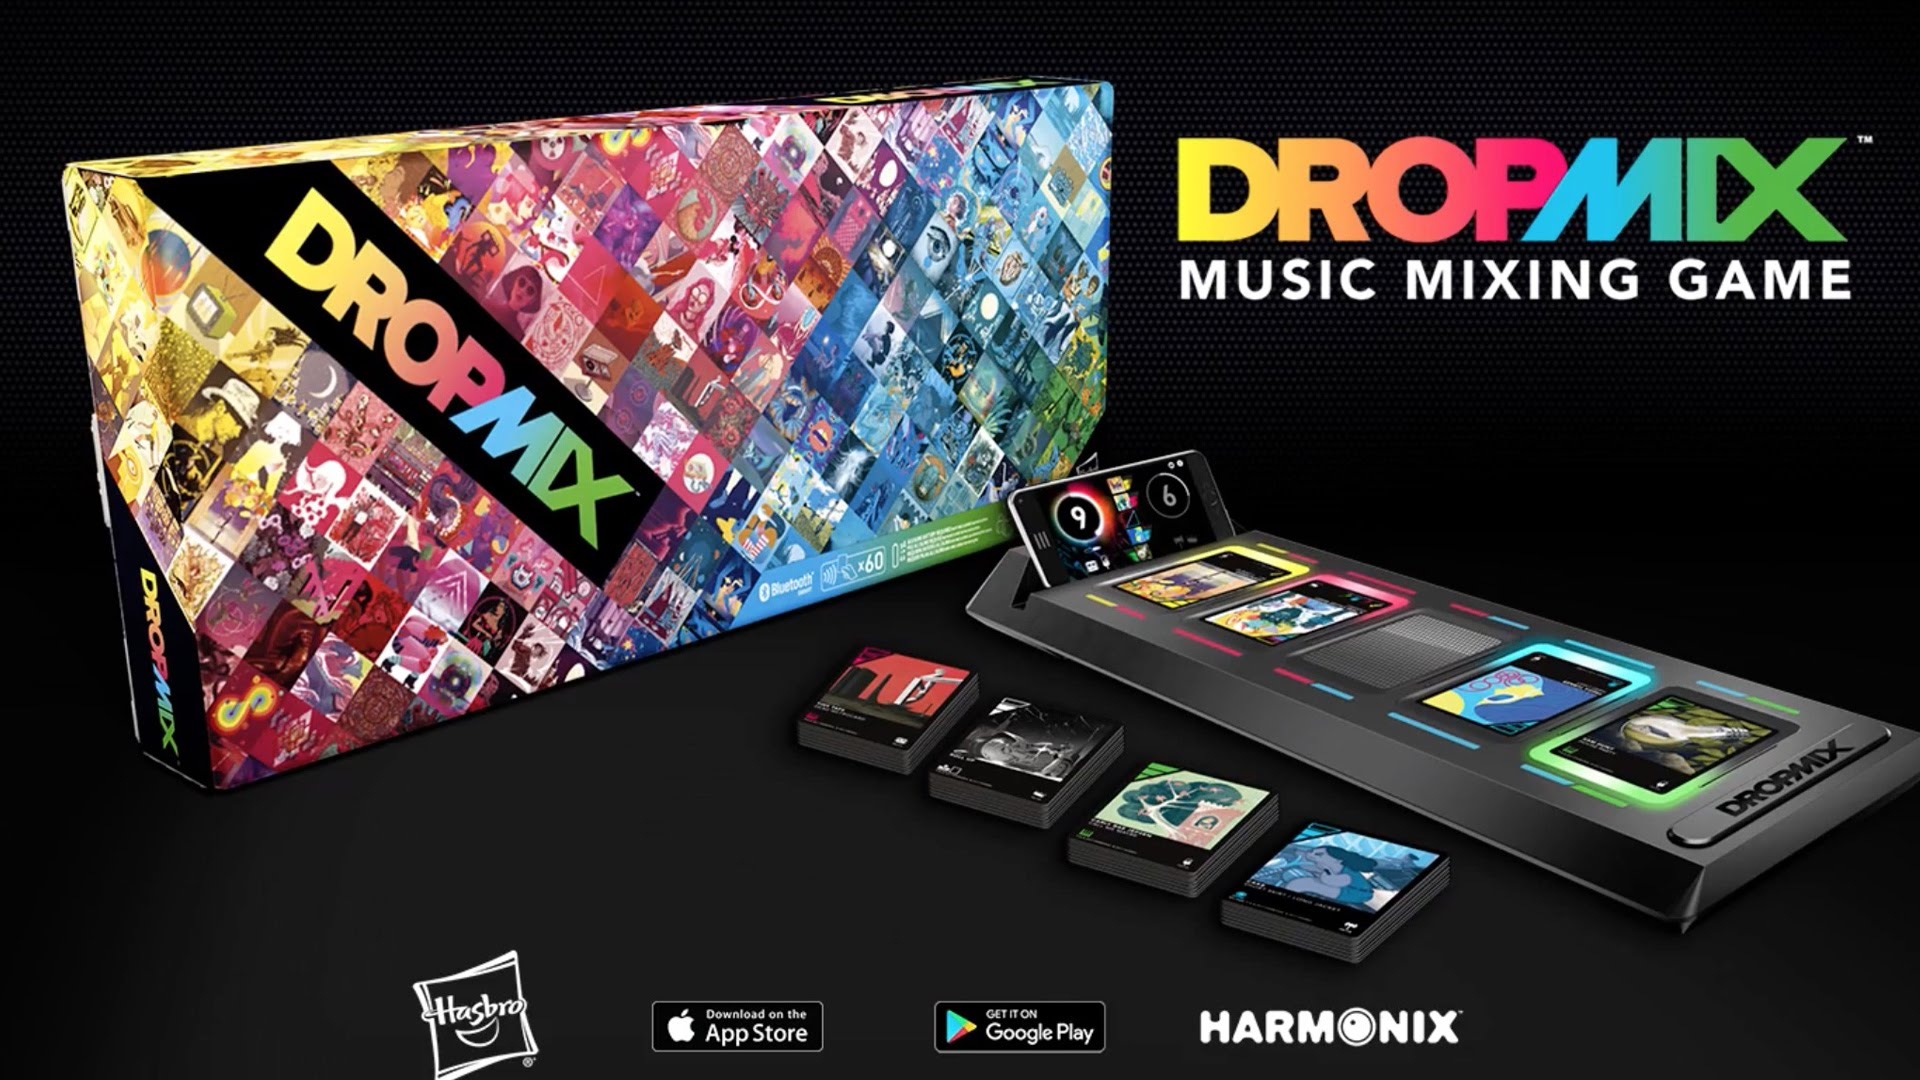
\includegraphics[width=0.7\linewidth]{figure/Analysis/dropmix}
	\label{fig:dropmix}
	\caption{Shows the Drop mix package \cite{DropmixPicture}}
\end{figure}


\subsection{Dance Dance Revolution}
DDR is a physical interactive dance platform created by the Japanese company Konami. Players will stand on this platform and press the colored arrows on the stand of the platform corresponding to the arrows that will be shown on the screen. Each player will then be judged on how they time their dance patterns. There are a variety of music to choose from and when picking one the screen will show arrows that the user must imitate on the platform to receive points. 

From the workshop it was found out that many of the children wants movement. This device gives the user the possibility of immersion by adding movement into learning. This device concentrates on music and dance. The device can be played together with other for adding more collaboration or it can be played alone. \cite{DanceDanceRevolution}

\begin{figure}[H]
	\centering
	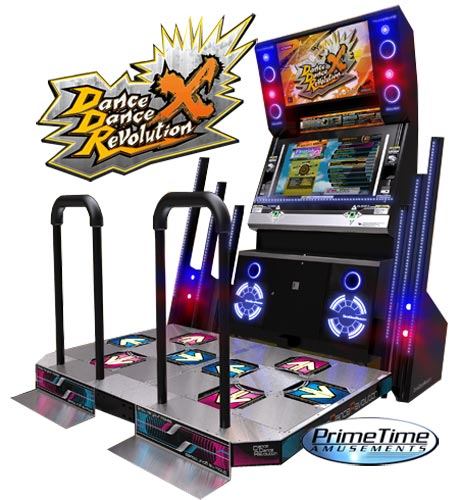
\includegraphics[width=0.7\linewidth]{figure/Analysis/dancedance}
	\label{fig:dancedance}
	\caption{shows the enlarged edition of Dance Dance Revolution, where the whole device is used for playing \cite{DanceDanceRevolutionPicture}}
\end{figure}

\subsection{Just dance}
Just dance is a dance video game developed by Ubisoft Milan and Ubisoft Paris. The game was released mainly for usage on Wii. The whole idea about the game is that each user must mimic the motions of an onscreen dancer’s choreography. For each movement the user will get more points and the more correct the movements are the more points the user will receive.

Just dance and Dance Dance Revolution are very similar. Just dance takes the idea about using the camera from Wii and utilizes this component. This also deletes the controversial problem about not having space enough because you can place the Wii anywhere. While the DDR is still a spacious device. As the workshop concludes it is very important for the children to be able to move and Just Dance adds the capability of moving freely around the room as long as the person is still within the range of the camera. \cite{JustDancenow}
\begin{figure}[H]
	\centering
	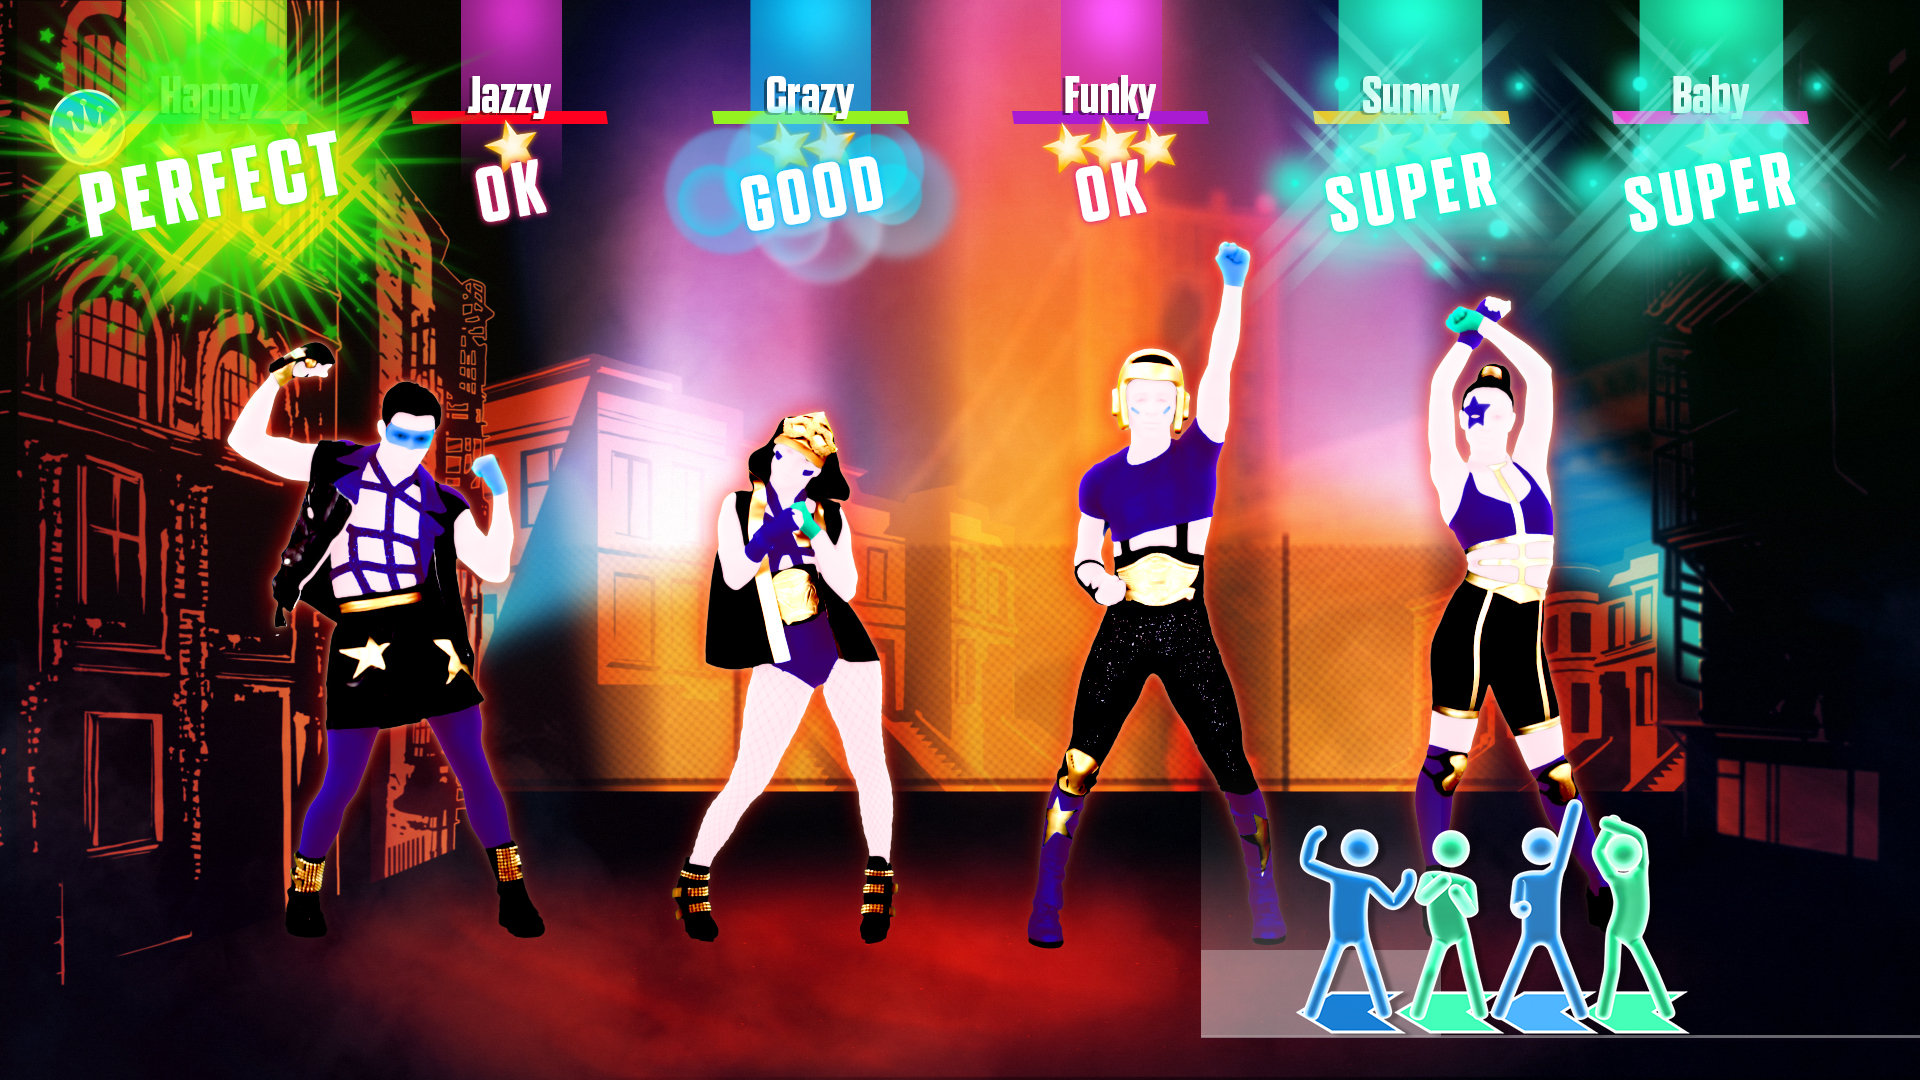
\includegraphics[width=0.7\linewidth]{figure/Analysis/justdance}
	\label{fig:Just Dance}
	\caption{Screen shot of how the game looks like \cite{JustDancenowPicture}}
\end{figure}

\subsection{Gridi}
Gridi is a physical board sequencer. Its purpose is to keep running on a loop and a matrix of 16x16 of different holes are placed on the board. Whenever a ball is placed in one of these holes the sequence changes the output and a different sound will be played. 

That makes Gridi a physical interactive interface that enables the user to make music by dropping some balls into each hole and removing them again as the user wish. This makes for a very interesting type of collaboration. It can be played by one but also as a group of people depending on how big the board is. \cite{Gridi}
\begin{figure}[H]
	\centering
	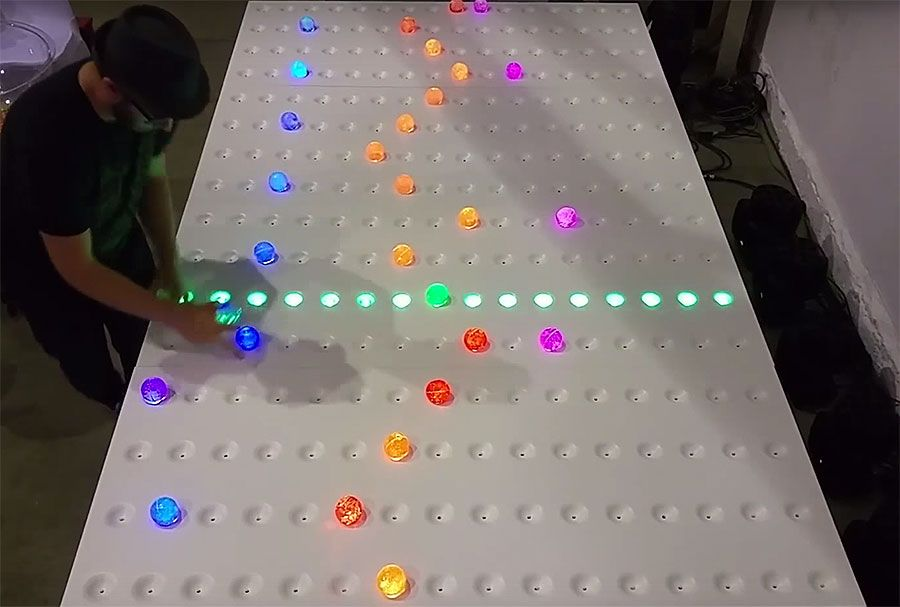
\includegraphics[width=0.7\linewidth]{figure/Analysis/gridi}
	\label{fig:Gridi}
	\caption{Shows the idea behind Gridi and how the loop and interactive balls works together \cite{GridiPicture}}
\end{figure}



	 
\subsection{State of the art sub conclusion}
All these devices given in State of the art states some good aspects of different components that can be used for further development of this reports design and implementation section. The themes found in the workshop are guidelines for what the target groups desired features are. These devices each uses some of the desired features or more. It was therefore found out that the target group needs are in use with what is already on the market. Taking each device into consideration when building the design requirements, it will give a foundation for providing this report with a solid understanding of movement, variation, games components, visuality and the understanding of components being physical. Taking from the state of the art, a device should have a concrete learning pattern that provides all learning patterns into consideration. It should visually be pleasing making the user want to interact more with the device. It would be a good idea to make it collaborative. The size only matters for which location the device is being positioned. Movement is a good option for making it more collaborative.

\todo{Make a summary of analysis}

\section{Final Problem Statement}\label{sec:FPS}
	How can a physical interface facilitate collaboration in small groups for elementary school children aged 8-12 years in a musical education context?
\todo{jeg synes (som stated i en anden kommentar), at FPSen skal placeres efter det afsnit der hedder "choice of direction" da det jo er med det afsnit vi kommer frem til vores FPS}
	
\section{Design Requirements}
	\subsection*{Functional Requirements}
		\begin{itemize}
			\item[-] It must accommodate at least 2 children.\\
			\item[-] It must accommodate max 6 children.\\
			\item[-] Must facilitate collaboration within at least one of the three musical areas of competence.\\
			\item[-] Must be designed for Children aged 8-12.\\
			\item[-] It should strive to not induce  negative emotions.\\
			\item[-] It should strive to induce positive emotions.\\
			\item[-] It must be designed for use in a classroom setting.\\
			\item[-] It must output sound.		
			
		\end{itemize}
	\subsection*{Non-Functional Requirements}
		\begin{itemize}
			\item[-] It must be interactable.\\
			\item[-] It must have a physical interface.\\
			\item[-] It must be drop resistant.\\
			\item[-] It must minimize unnecessary noise.
		\end{itemize}
	
















		